\documentclass[tikz,border=8pt]{standalone}
\usepackage{amsmath}
\usetikzlibrary{arrows.meta}

\begin{document}
\sffamily
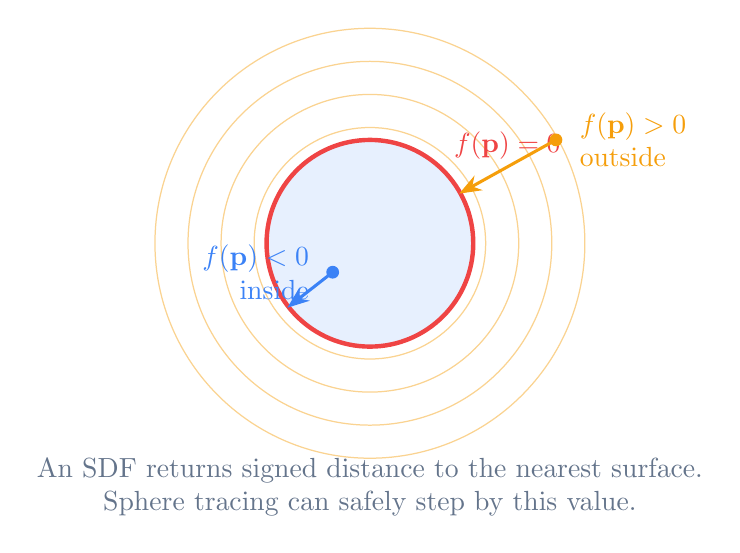
\begin{tikzpicture}[scale=1.05, >=Stealth]
  \definecolor{inside}{RGB}{59,130,246}
  \definecolor{outside}{RGB}{245,158,11}
  \definecolor{surface}{RGB}{239,68,68}
  \definecolor{softgray}{RGB}{100,116,139}

  \foreach \r in {0.6,1.0,1.4,1.8,2.2,2.6} {
    \draw[outside!45, line width=0.45pt] (0,0) circle (\r);
  }
  \fill[inside!12] (0,0) circle (1.25);
  \draw[surface, line width=1.6pt] (0,0) circle (1.25);
  \node[surface, above right] at (0.9,0.9) {$f(\mathbf{p})=0$};

  \coordinate (Pout) at (2.25,1.25);
  \coordinate (Pin) at (-0.45,-0.35);
  \fill[outside] (Pout) circle (2.2pt);
  \fill[inside] (Pin) circle (2.2pt);
  \draw[outside, ->, line width=1.1pt] (Pout) -- (1.08,0.60);
  \draw[inside, ->, line width=1.1pt] (Pin) -- (-1.0,-0.78);

  \node[outside, right, align=left] at (2.42,1.25) {$f(\mathbf{p})>0$\\outside};
  \node[inside, left, align=right] at (-0.62,-0.35) {$f(\mathbf{p})<0$\\inside};

  \node[softgray, align=center] at (0,-2.95)
    {An SDF returns signed distance to the nearest surface.\\Sphere tracing can safely step by this value.};
\end{tikzpicture}
\end{document}
